\documentclass[a4paper, 12pt]{article}

%%% SST LAB PROTOCOLL PREAMBLE
%%% 2019
%%%%%%%%%%%%%%%%%%%%%%%%%%%%%%%


%%% PACKAGES
%%%%%%%%%%%%%%%%%%%%%%%%%%%

\usepackage[ngerman]{babel}

\usepackage[utf8]{inputenc}
\usepackage{amsmath}
\usepackage{pgfplots}
\usepackage{tikz}
\usepackage[many]{tcolorbox}
\usepackage{graphicx}
\graphicspath{ {./graphics/} }
\usepackage{pdfpages}
\usepackage{dashrule}
\usepackage{float}
\usepackage{siunitx}
\usepackage{trfsigns}
\usepackage{booktabs}
\usepackage[european]{circuitikz}
\usepackage{tcolorbox}

%%% DOCUMENT GEOMETRY
%%%%%%%%%%%%%%%%%%%%%%%%%%%

\usepackage{geometry}
\geometry{
 a4paper,
 total={0.6180339887498948\paperwidth,0.6180339887498948\paperheight},
 top = 0.1458980337503154\paperheight,
 bottom = 0.1458980337503154\paperheight
 }
\setlength{\jot}{0.013155617496424828\paperheight}
\linespread{1.1458980337503154}

\setlength{\parskip}{0.013155617496424828\paperheight} % paragraph spacing


%%% COLORS
%%%%%%%%%%%%%%%%%%%%%%%%%%%

\definecolor{red1}{HTML}{f38181}
\definecolor{yellow1}{HTML}{fce38a}
\definecolor{green1}{HTML}{95e1d3}
\definecolor{blue1}{HTML}{66bfbf}
\definecolor{hsblue}{HTML}{00b1db}
\definecolor{hsgrey}{HTML}{afafaf}

%%% CONSTANTS
%%%%%%%%%%%%%%%%%%%%%%%%%%%
\newlength{\smallvert}
\setlength{\smallvert}{0.0131556\paperheight}


%%% COMMANDS
%%%%%%%%%%%%%%%%%%%%%%%%%%%

% differential d
\newcommand*\dif{\mathop{}\!\mathrm{d}}

% horizontal line
\newcommand{\holine}[1]{
  	\begin{center}
	  	\noindent{\color{hsgrey}\hdashrule[0ex]{#1}{1pt}{3mm}}\\%[0.0131556\paperheight]
  	\end{center}
}

% mini section
\newcommand{\minisec}[1]{ \noindent\underline{\textit {#1} } \\}

% quick function plot
\newcommand{\plotfun}[3]{
  \vspace{0.021286\paperheight}
  \begin{center}
    \begin{tikzpicture}
      \begin{axis}[
        axis x line=center,
        axis y line=center,
        ]
        \addplot[draw=red1][domain=#2:#3]{#1};
      \end{axis}
    \end{tikzpicture}
  \end{center}
}

% box for notes
\newcommand{\notebox}[1]{

\tcbset{colback=white,colframe=green1!100!black,title=Note!,width=0.618\paperwidth,arc=0pt}

 \begin{center}
  \begin{tcolorbox}[]
   #1 
  \end{tcolorbox}
 
 \end{center} 
 
}

% box for equation
\newcommand{\eqbox}[2]{
	
	\tcbset{colback=white,colframe=green1!100!black,title=,width=#2,arc=0pt}
	
	\begin{center}
		\begin{tcolorbox}[ams align*]
				#1
		\end{tcolorbox}
		
	\end{center} 
	
}
% END OF PREAMBLE

%%%%%%%%%%%%%%%%%%%%%%%%%%%%%%%%%%%%%

\begin{document}

%%%%%%%%%%%%%%%%%%%%%%%%%%%%%%%%%%%%%
  
\includepdf{./titlepage/titlepage.pdf}
  \clearpage
  \setcounter{page}{1}
%%%%%%%%%%%%%%%%%%%%%%%%%%%%%%%%%%%%%

\section{Vorbereitungsaufgaben}

\subsection{}
\begin{figure}[H]
	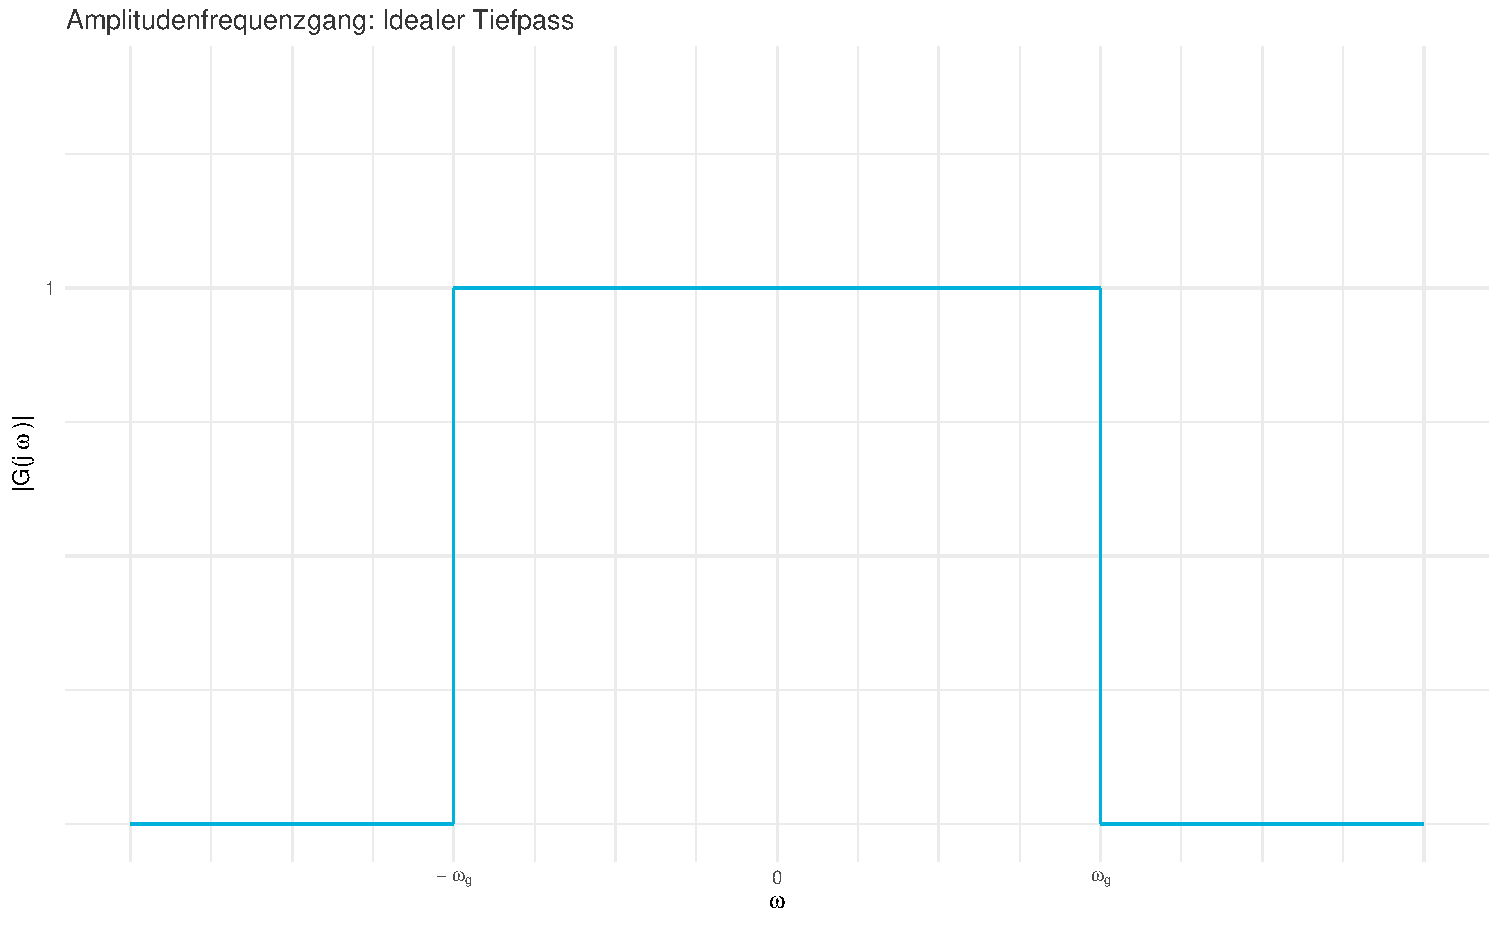
\includegraphics[width=\textwidth]{1_1/TP_ideal}
\end{figure}

\begin{figure}[H]
	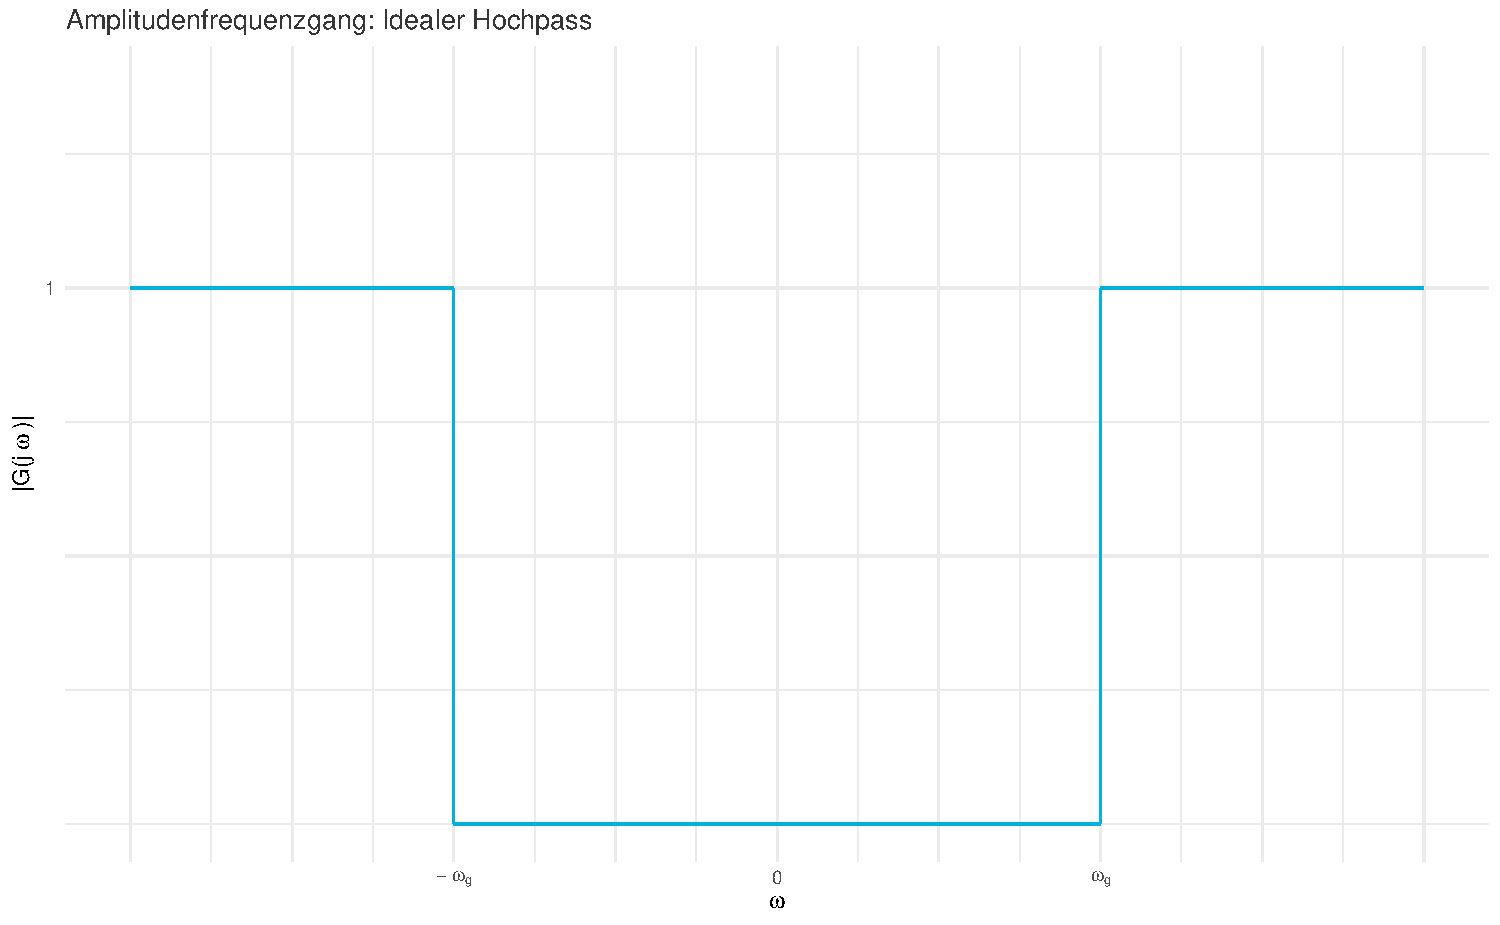
\includegraphics[width=\textwidth]{1_1/HP_ideal}
\end{figure}

\begin{figure}[H]
	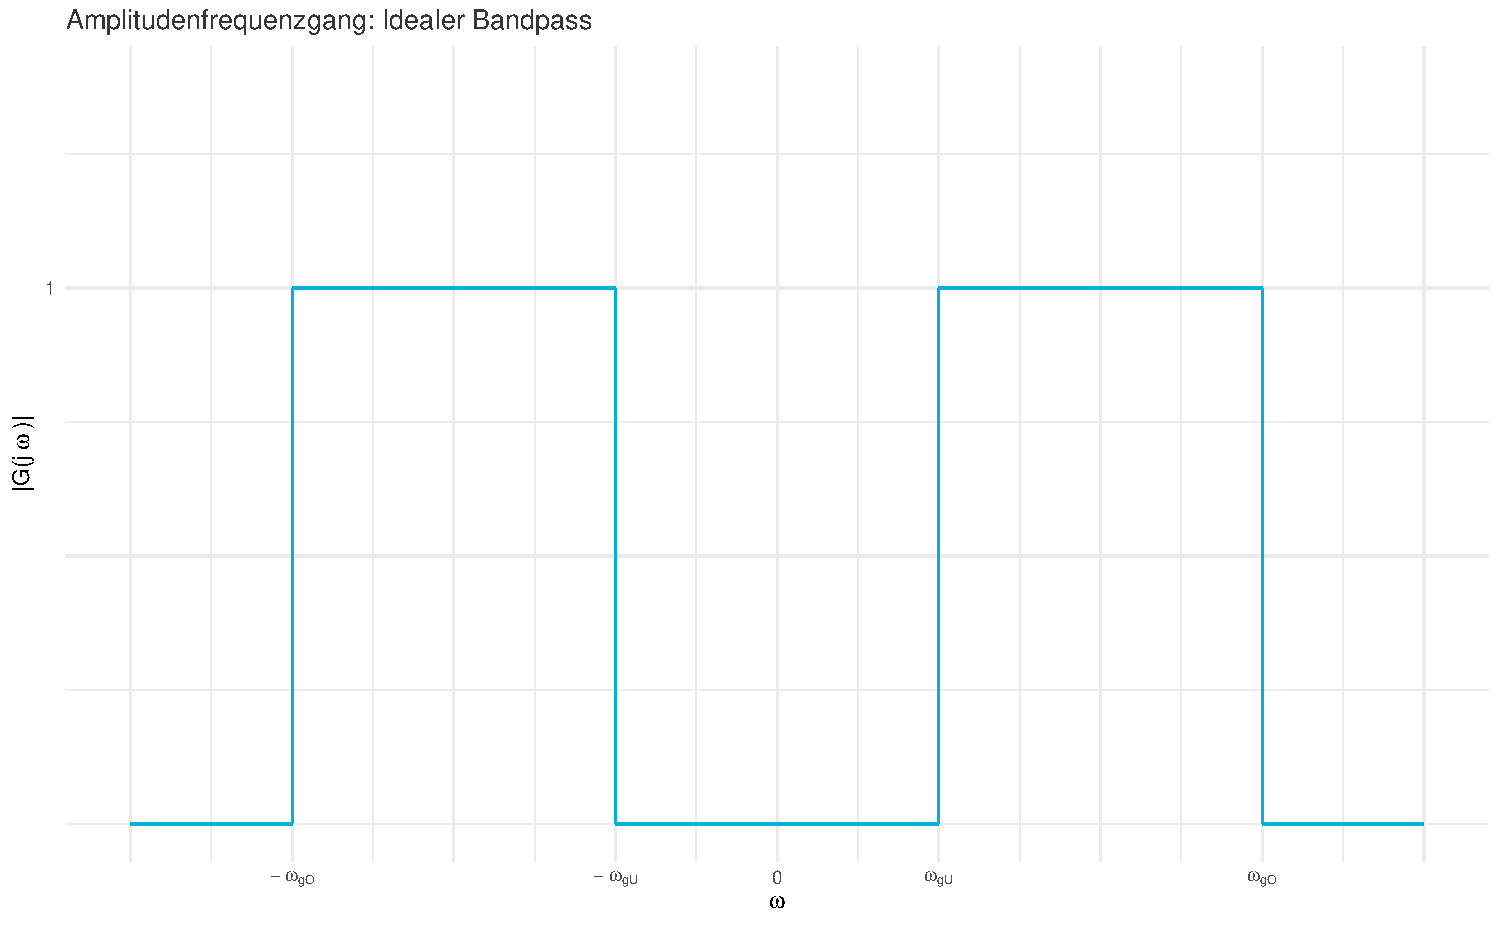
\includegraphics[width=\textwidth]{1_1/BP_ideal}
\end{figure}

\subsection{}

\begin{figure}[H]
	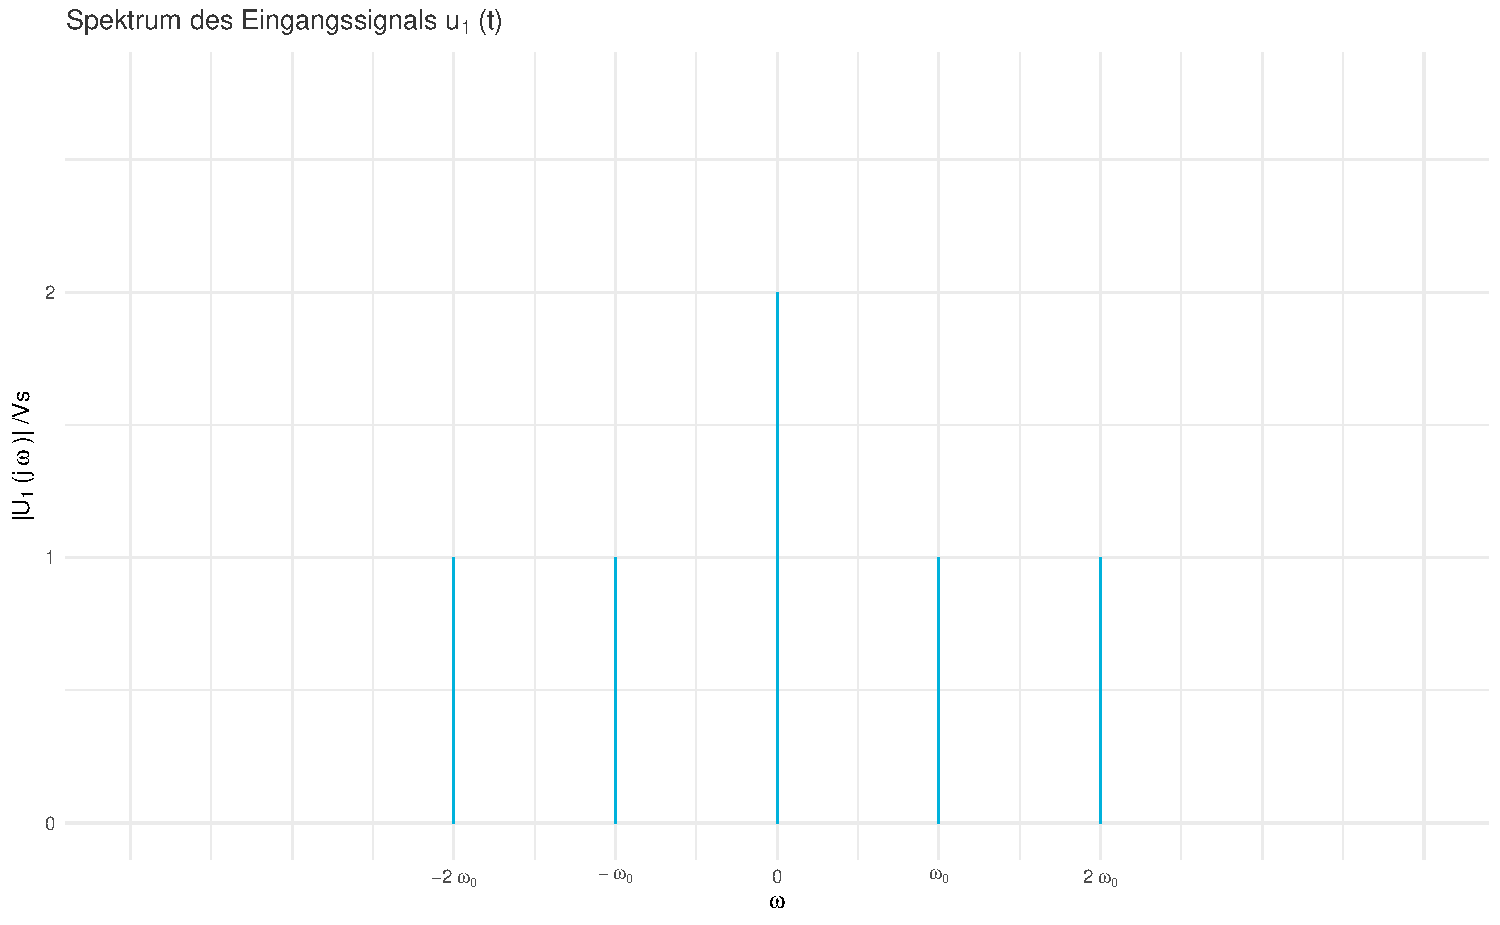
\includegraphics[width=\textwidth]{1_2/TP}
\end{figure}

\begin{figure}[H]
	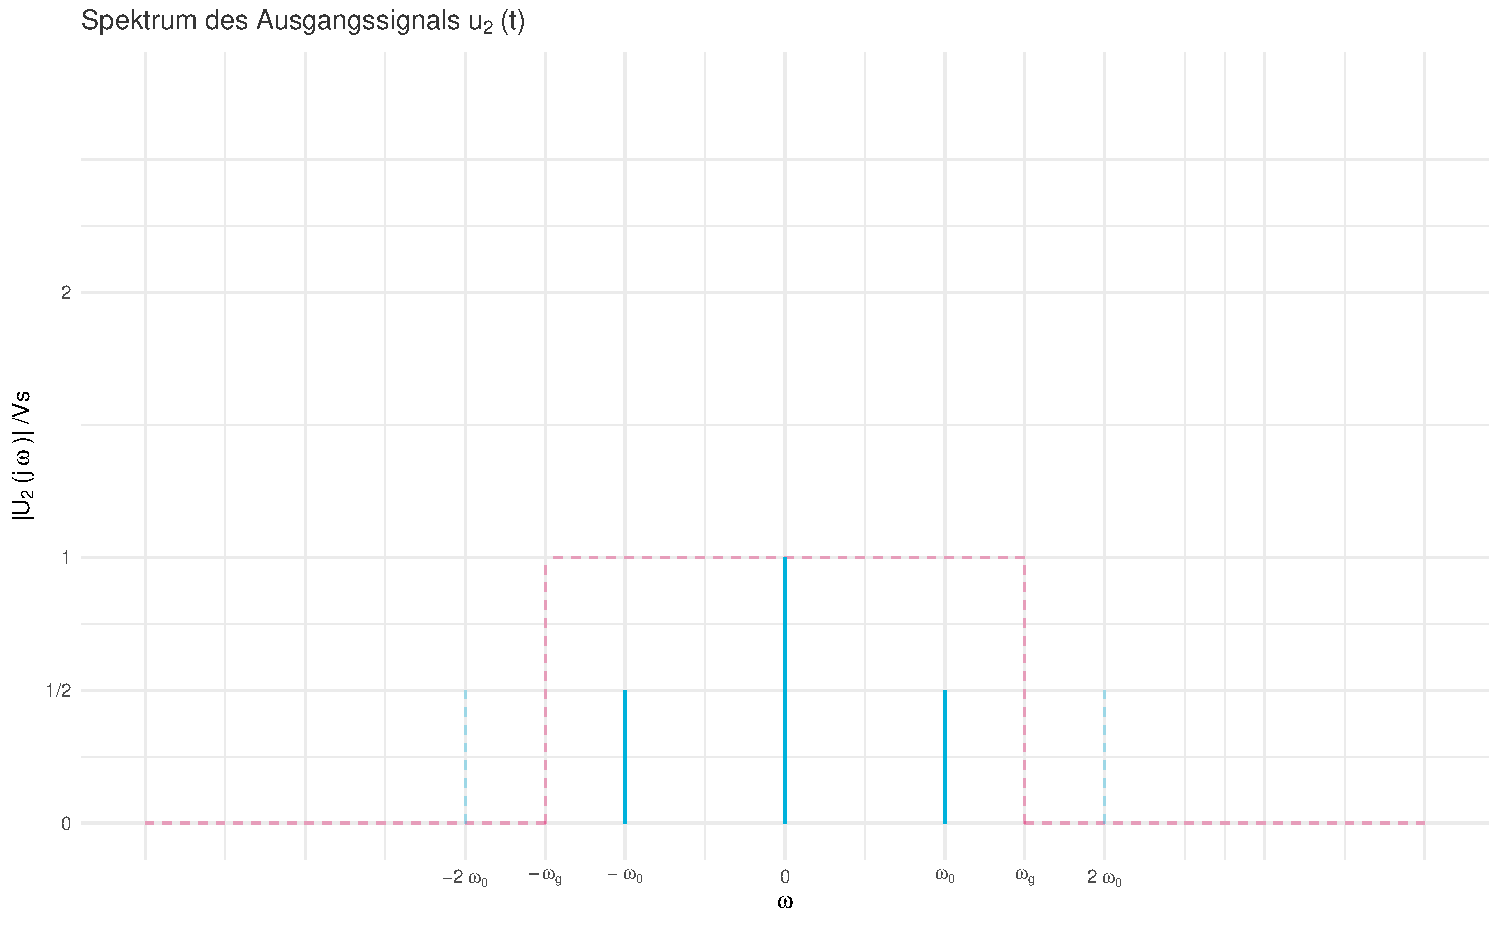
\includegraphics[width=\textwidth]{1_2/Ausgangsspektrum}
\end{figure}


Aus der grafischen Betrachtung der Spektren von Ein- und Ausgangssignal und
unter Berücksichtigung der Übergangsfunktion des Tiefpasses lässt sich erkennen,
dass die Grenzfrequenz des Tiefpasses zwischen $\omega_0$ und $2 \,\omega_0$
liegen muss, um den Frequenzanteil bei $\omega_0$ durchzulassen und bei
$2\,\omega_0$ auszulöschen. Der Faktor $K_1$ ist durch die Skalierung der
Amplitude beim Durchlauf des Tiefpasses gleich $1/2$.

Der Parameter $\phi$ beschreibt die Phasenverschiebung vom Ausgangssignal zum
Eingangssignal, welche sich beim idealen Tiefpass linear mit der Frequenz
ändert. Im Zeitbereich erkennt man dadurch eine Zeitverschiebung $t_0$, wodurch
$\phi = \omega_0 \cdot t_0$.

\subsection{}
Das System kann lineare Verzerrungen hervorrufen, da es Frequenzanteile
unterdrücken oder durchlassen kann.

\subsection{}
Zufällige Signale können durch ihre \emph{Autokorrelation}, welche die Änhlichkeit eines
Signals mit sich selbst ausdrückt, charakterisiert werden. Idealerweise ist
diese Ähnlichkeit bei zufälligen Signalen bei jeder Verschiebung ungleich 0 nicht gegeben.

Ideales gaußverteiltes Rauschen besitzt zudem ein \emph{konstantes
Leistungsdichtespektrum}.

\subsection{}

Idealerweise kann die Übertragungsfunktion eines Systems durch Anregung des
Systems mit einem \emph{Dirac-Impuls} im Zeitbereich bestimmt werden. Der Dirac-Impuls
besitzt im Frequenzbereich eine konstante Amplitude (1) über alle Frequenzen.
Die Auswertung im Frequenzbereich ergibt daher (mit $\Delta(j\omega) = \mathcal{F} (\delta(t))$):
$$ U_2(j \omega) = G(j \omega) \cdot U_1(j \omega) = G(j \omega) \cdot \Delta(j
\omega) = G(j \omega)$$

Der demnach ermittelte Betragsgang am Ausgang ist somit gleich der
Übertragungsfunktion des Systems. Praktisch ist diese Methode jedoch kaum
möglich, da es schwierig ist, einen zeitlich unendlich kurzen Impuls von
unendlicher Amplitude (hohe Energie) zu
erzeugen und gleichzeitig Nichtlinearitäten,
Trägheit/Verzögerungen und Belastbarkeit des zu messenden Systems zu berücksichtigen.

Als praktischere Alternative zum Dirac-Impuls kann man einen \emph{Sprung} der Höhe 1 auf das System geben und mit der \emph{Sprungantwort} am Ausgang des Systems die Übertragungsfunktion feststellen.

Eine weitere Möglichkeit ist die diskrete Analyse des Systems bei bestimmten
Frequenzen, z.B. durch Anregung mit einem \emph{Wobble-Sinus} und die Aufnahme von
Messpunkten in geeigneten Abständen. Nachteil ist hier die begrenzte Auflösung.

\section{Versuchsaufgaben}

\subsection{Analyse von Filterschaltungen}

In der ersten Versuchsaufgabe wurden die Spannungsamplituden $U_2$ der Ausgangssignale der in
Box 3 enthaltenen 4 Filterschaltungen bei sinusförmigem Eingangssignal mit einer
Amplitude von $1 \, \si{\volt}$ mit dem Oszilloskop gemessen. Das
Amplitudenverhältnis $U_2/U_1$ wurde anschließend in $\si{\deci\bel}$
ausgedrückt, um einfache Aussagen über die jeweilige Grenzfrequenz und Filterordnung treffen zu können.

\subsubsection{Box3.1}
\begin{table}[H]
  \begin{center}
    \begin{tabular}{@{}rrr@{}}
      \toprule
      $f / \si{\hertz}$ & $U_2 / \si{\milli\volt}$ & $U_2/U_1 / \si{\deci\bel}$ \\ \midrule
      500               & 1084                     & 0.70                       \\
      2000              & 1061                     & 0.51                       \\
      4000              & 1000                     & 0.00                       \\
      8000              & 826                      & -1.66                      \\
      10000             & 750                      & -2.50                      \\
      11300             & 699                      & -3.11                      \\
      12000             & 688                      & -3.25                      \\
      14000             & 627                      & -4.05                      \\
      20000             & 492                      & -6.16                      \\
      60000             & 230                      & -12.77                     \\
      80000             & 180                      & -14.89                     \\
      100000            & 130                      & -17.72                     \\
      200000            & 131                      & -17.65                     \\
      300000            & 129                      & -17.79                     \\
      400000            & 123                      & -18.20                     \\
      1000000           & 97                       & -20.26                     \\ \bottomrule
    \end{tabular}
    \end{center}
    \caption{Messwerte des ersten Filters der Box 3}
\end{table}

\begin{figure}[H]
	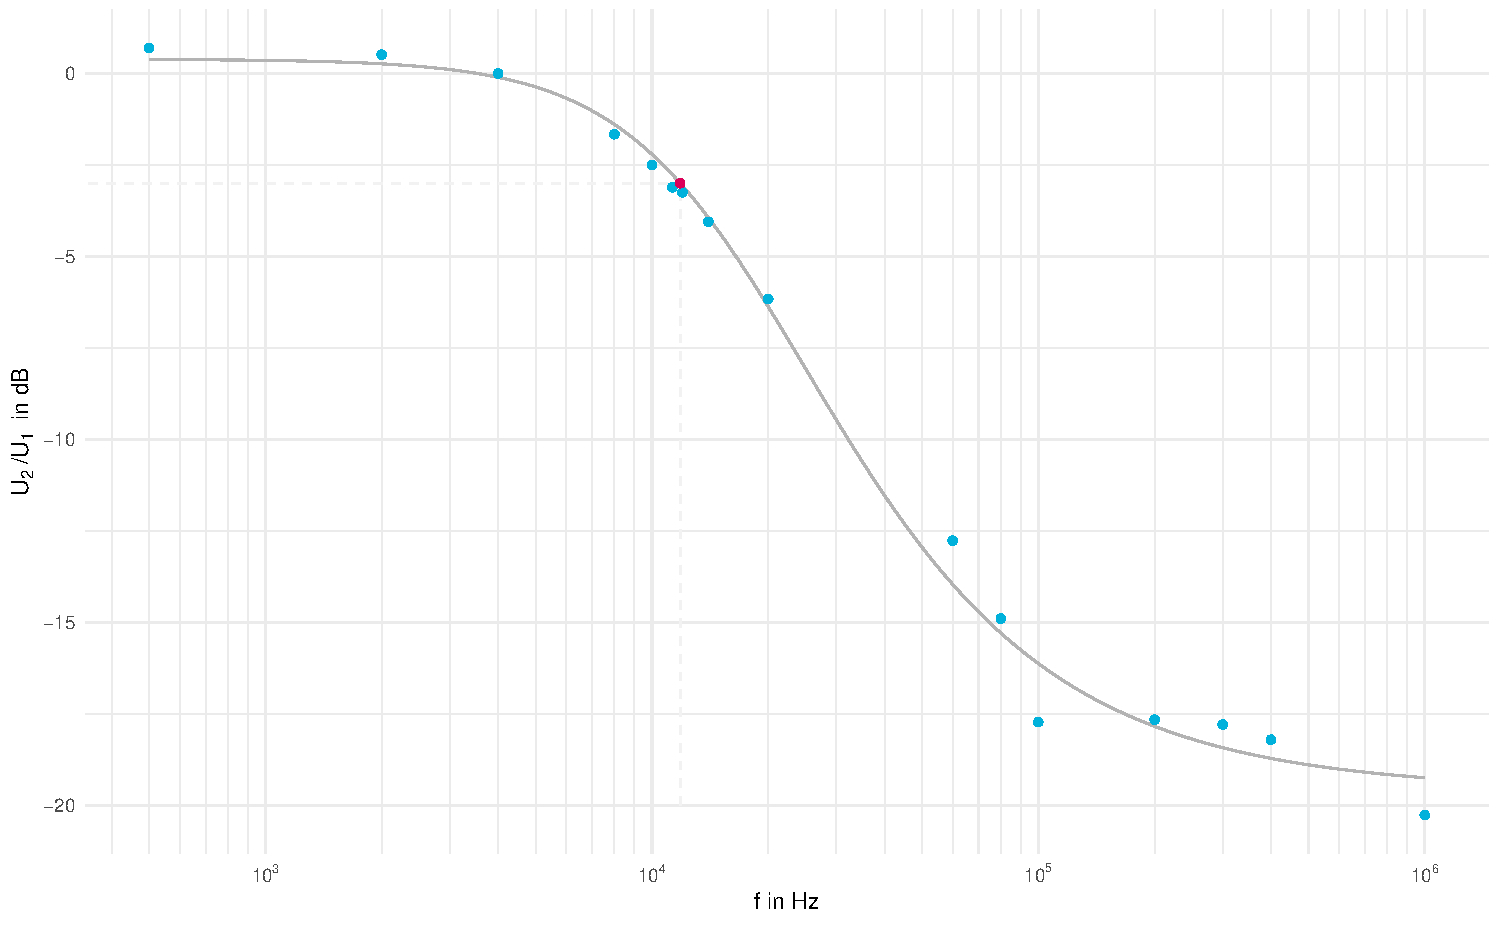
\includegraphics[width=\textwidth]{Messwerte/Box3-1/Box3-1}
  \caption{Bodediagramm Box3.1}
\end{figure}

Bei der Versuchsdurchführung wurden die Frequenzen der Messpunkte um die
Grenzfrequenz herum gewählt, welche vorher für jedes Filter durch Messung einer
Amplitude von etwa $707 \, \si{\milli\volt}$, also $1/\sqrt{2}$ der
Eingangsamplitude, gemessen wurde.  

Aus Abbildung 1 lässt sich erkennen, dass es sich
bei der ersten Schaltung um ein Tiefpassfilter handelt. Die Grenzfrequenz des
Filters wurde nachträglich mittels Regression (Modellgleichung der Form $u(f) = a + b/\sqrt{1
  + (k \cdot f)^2}$) bei einer Dämpfung der Amplitude von $3 \, \si{\deci\bel}$ bestimmt.

$$f_{\textrm{g}_{3.1}} = 11837 \,\ \si{\hertz}$$

Handschriftlich wurde dann durch Linearisierung des Filterverlaufs die Filterordnung
über die Geradensteigung bestimmt (Bei TP n-ter Ordnung circa $-n\cdot 20 \,
\si{\deci\bel}/\textrm{Dekade}$ nach der Grenzfrequenz). Die roten Punkte
kennzeichnen jeweils den Filterwert von $-3 \, \si{\deci\bel}$ bei der Grenzfrequenz.
 
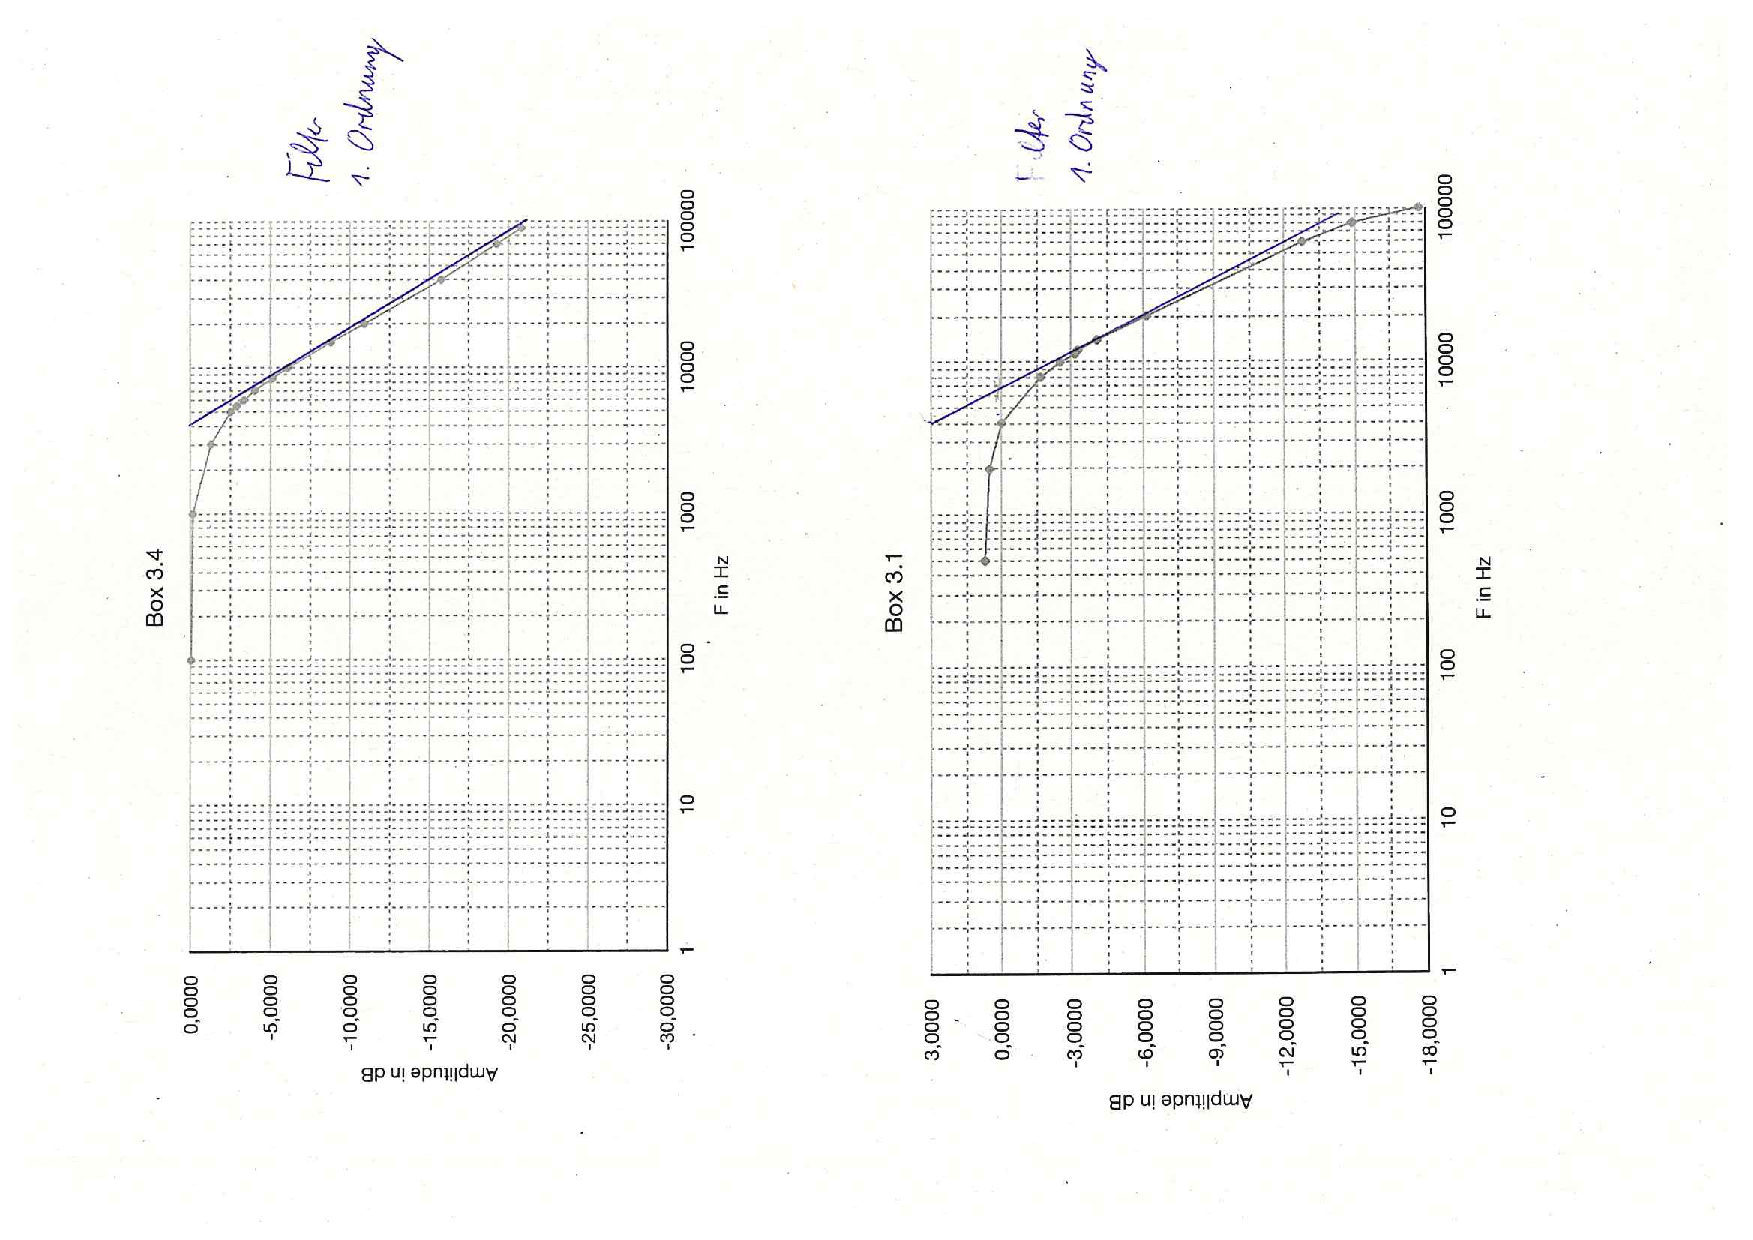
\includepdf[pages={1-}, angle=-90]{Messwerte/Filterscan}

\subsubsection{Box3.2}

\begin{table}[H]
  \begin{center}
    \begin{tabular}{@{}rrr@{}}
      \toprule
      $f / \si{\hertz}$ & $U_2 / \si{\milli\volt}$ & $U_2/U_1 / \si{\deci\bel}$ \\ \midrule
      100   & 69  & -23.22 \\
      200   & 123 & -18.20 \\
      300   & 168 & -15.49 \\
      600   & 290 & -10.75 \\
      1000  & 433 & -7.27  \\
      1500  & 579 & -4.75  \\
      2000  & 687 & -3.26  \\
      2300  & 727 & -2.77  \\
      5000  & 912 & -0.80  \\
      10000 & 951 & -0.44  \\
      15000 & 978 & -0.19  \\ \bottomrule
    \end{tabular}
    \end{center}
    \caption{Messwerte des zweiten Filters der Box 3}
\end{table}

\begin{figure}[H]
	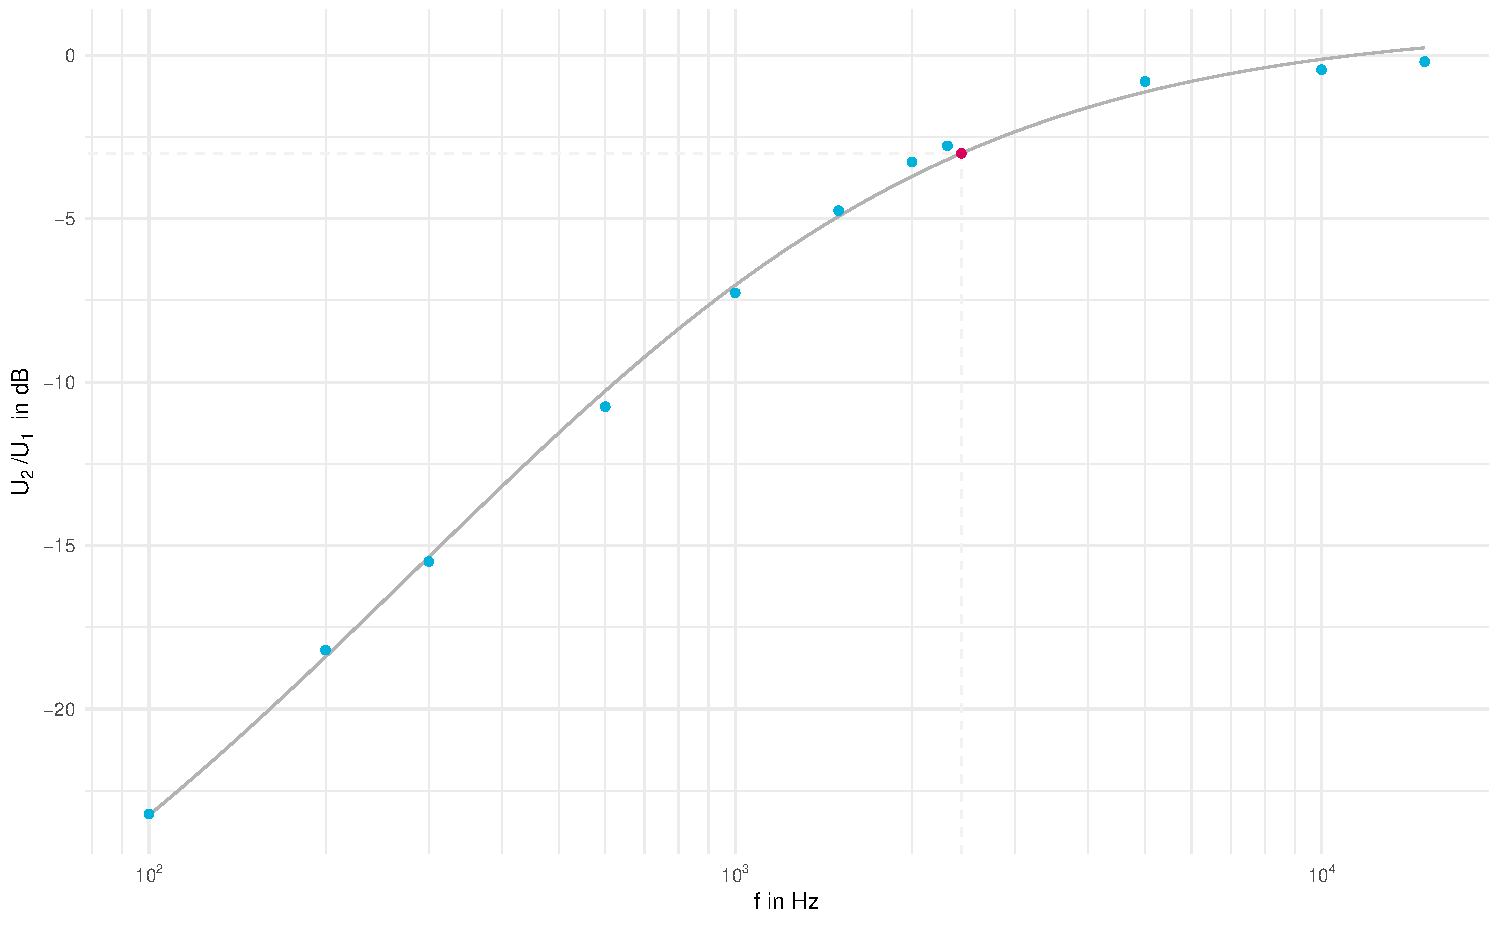
\includegraphics[width=\textwidth]{Messwerte/Box3-2/Box3-2}
  \caption{Bodediagramm Box3.2}
\end{figure}
Box3.2 ist, wie in Abbildung 2 zu erkennen, ein Hochpassfilter.
Die Grenzfrequenz ist
$$f_{\textrm{g}_{3.2}} = 2430 \,\ \si{\hertz}$$

\subsubsection{Box3.3}

\begin{table}[H]
  \begin{center}
    \begin{tabular}{@{}rrr@{}}
      \toprule
      $f / \si{\hertz}$ & $U_2 / \si{\milli\volt}$ & $U_2/U_1 / \si{\deci\bel}$ \\ \midrule
      1     & 988 & -0.10\\
      500   & 936 & -0.57\\
      700   & 882 & -1.09\\
      1000  & 815 & -1.78\\
      1200  & 777 & -2.19\\
      1500  & 705 & -3.04\\
      2000  & 600 & -4.44\\
      3000  & 456 & -6.82\\
      6000  & 257 & -11.80\\
      10000 & 169 & -15.44\\
      20000 & 102 & -19.83\\
      30000 & 69  & -23.22\\ \bottomrule
    \end{tabular}
  \end{center}
  \caption{Messwerte des dritten Filters der Box 3}
\end{table}

\begin{figure}[H]
	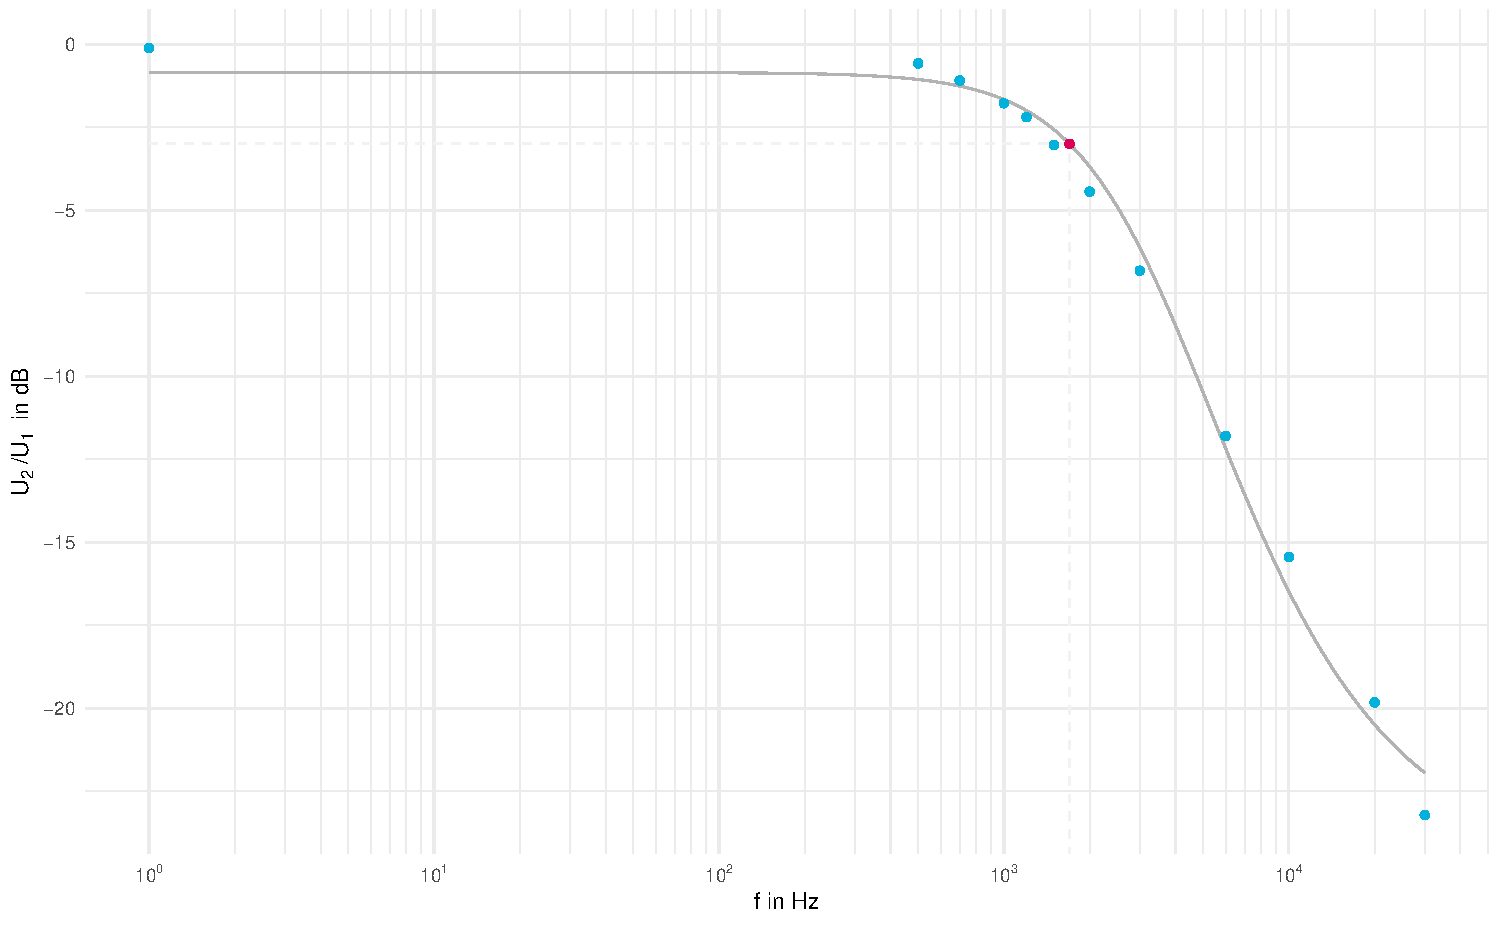
\includegraphics[width=\textwidth]{Messwerte/Box3-3/Box3-3}
  \caption{Bodediagramm Box3.3}
\end{figure}

Box3.3 ist, wie in Abbildung 3 zu erkennen, ein Tiefpassfilter.
Die Grenzfrequenz ist
$$f_{\textrm{g}_{3.3}} =  1700 \,\ \si{\hertz}$$

\subsubsection{Box3.4}

\begin{table}[H]
  \begin{center}
    \begin{tabular}{@{}rrr@{}}
      \toprule
      $f / \si{\hertz}$ & $U_2 / \si{\milli\volt}$ & $U_2/U_1 / \si{\deci\bel}$ \\ \midrule
      100   & 997 & -0.04\\
      1000  & 984 & -0.14\\
      3000  & 865 & -1.26\\
      5000  & 750 & -2.50\\
      5500  & 717 & -2.89\\
      6000  & 682 & -3.32\\
      7000  & 630 & -4.01\\
      8500  & 555 & -5.11\\
      10000 & 496 & -6.09\\
      15000 & 363 & -8.80\\
      20000 & 285 & -10.90\\
      40000 & 163 & -15.76\\
      70000 & 109 & -19.25\\
      90000 & 91  & -20.82\\ \bottomrule
    \end{tabular}
  \end{center}
  \caption{Messwerte des vierten Filters der Box 3}
\end{table}

\begin{figure}[H]
	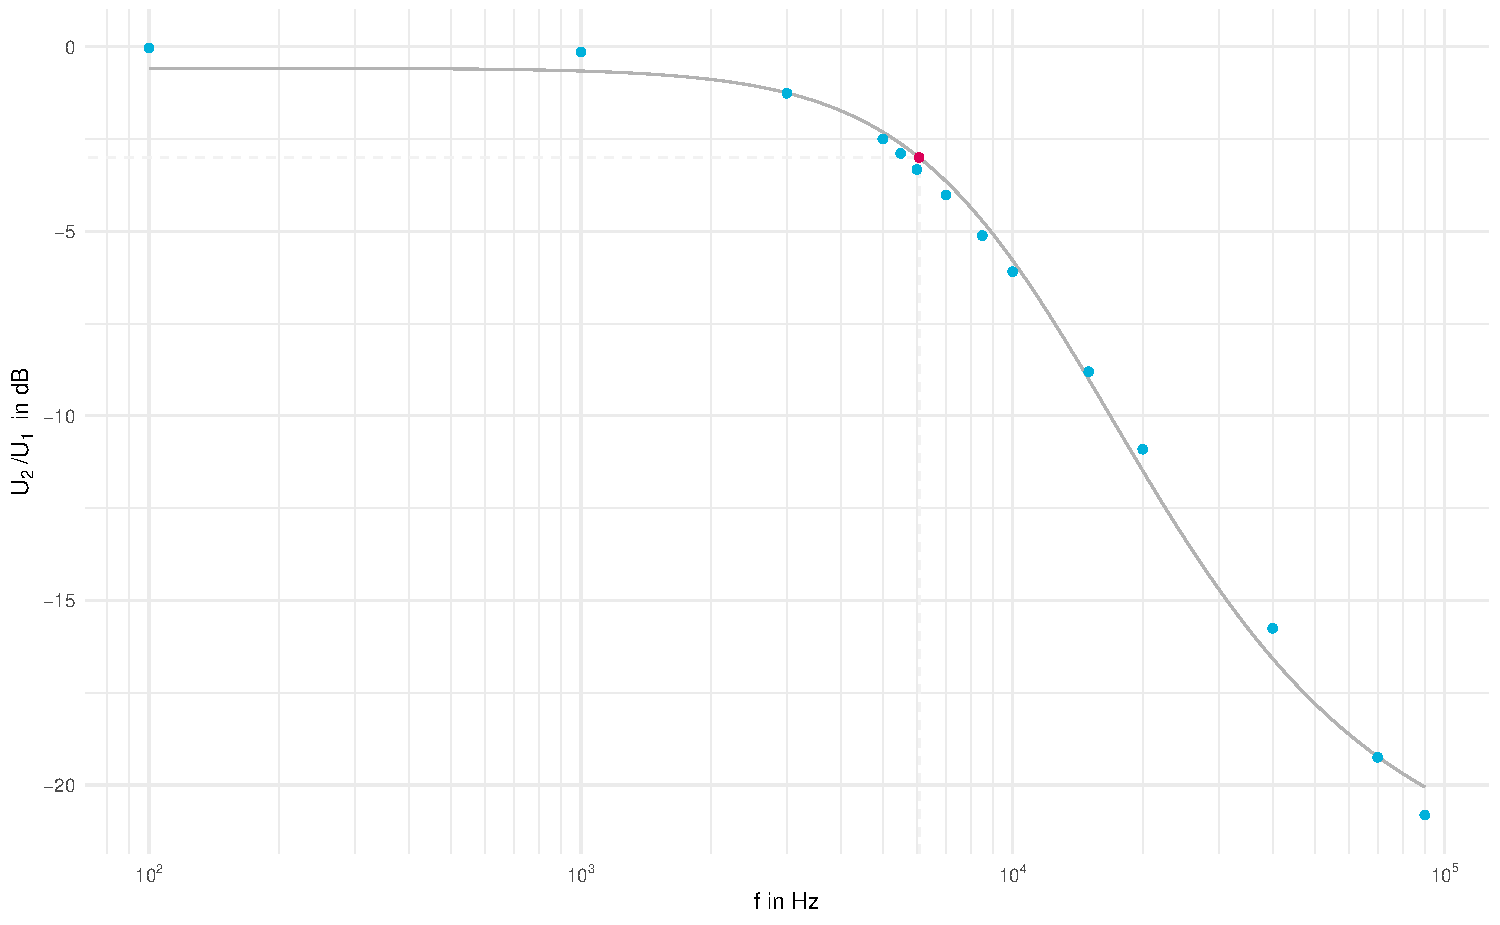
\includegraphics[width=\textwidth]{Messwerte/Box3-4/Box3-4}
  \caption{Bodediagramm Box3.4}
\end{figure}

Box3.4 ist, wie in Abbildung 4 zu erkennen, ein Tiefpassfilter.
Die Grenzfrequenz ist
$$f_{\textrm{g}_{3.4}} =  6070 \,\ \si{\hertz}$$


\subsection{Rauschsignal an den Filtereingängen}

\begin{figure}[H]
	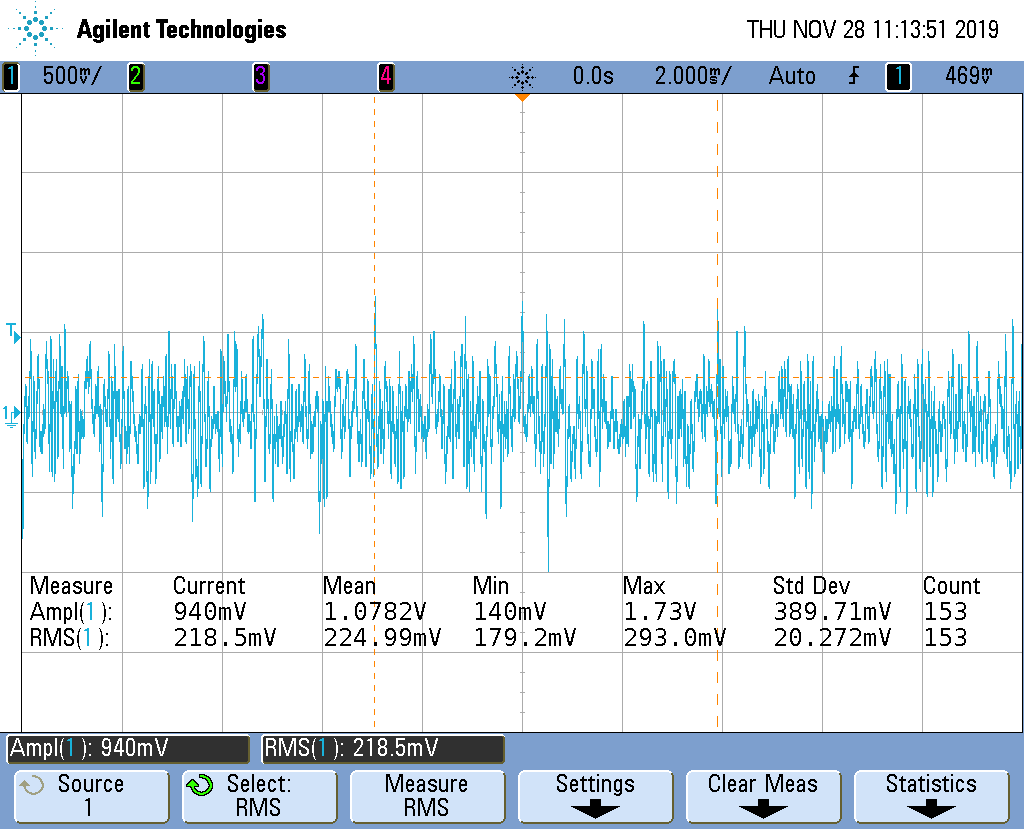
\includegraphics[width=\textwidth]{Messwerte/Rauschen/Rauschen_blue}
  \caption{Screenshot des verwendeten Rauschsignals}
\end{figure}

Das Rauschsignal wurde mithilfe eines MATLAB-Scripts erzeugt und an die Eingänge
der Tiefpassfilterschaltungen von Box 3 gelegt. Mit dem Oszilloskop wurde der
Effektivspannungswert der Ausgangssignale gemessen. Durch Quadrieren dieser
Werte konnte dann ein Maß für die Rauschleistung geschaffen werden, welche dann
über die jeweiligen Grenzfrequenzen der Filterschaltungen aufgetragen wurde.

\begin{figure}[H]
\begin{center}
	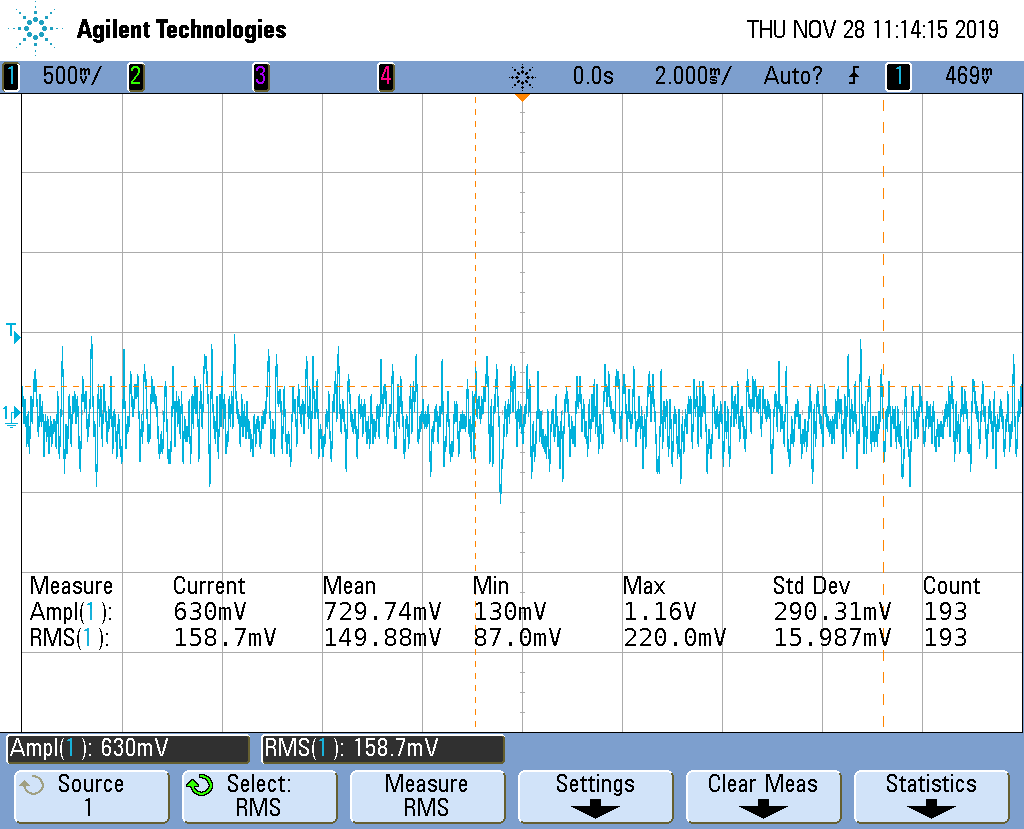
\includegraphics[height=0.618\textwidth]{Messwerte/Rauschen/Box1_blue}
  \caption{Screenshot des Ausgangssignals von Box3.1}
  \end{center}
\end{figure}

\begin{figure}[H]
  \begin{center}
	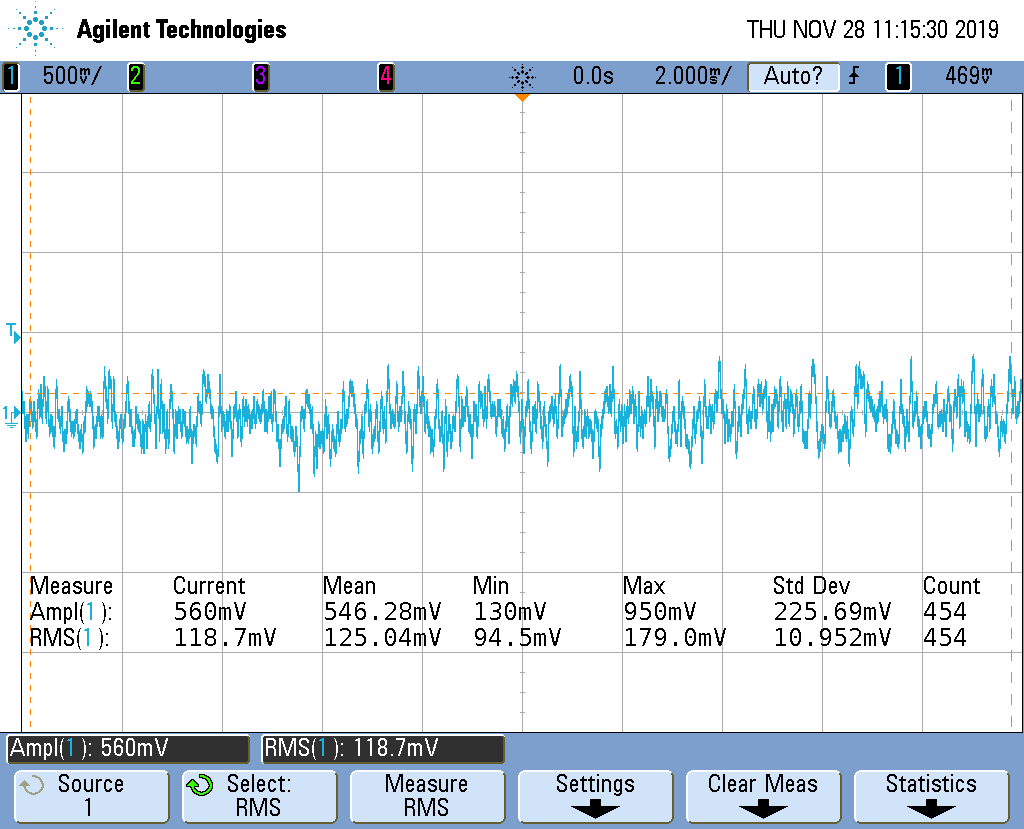
\includegraphics[height=0.618\textwidth]{Messwerte/Rauschen/Box3_blue}
  \caption{Screenshot des Ausgangssignals von Box3.3}
\end{center}
\end{figure}

\begin{figure}[H]
	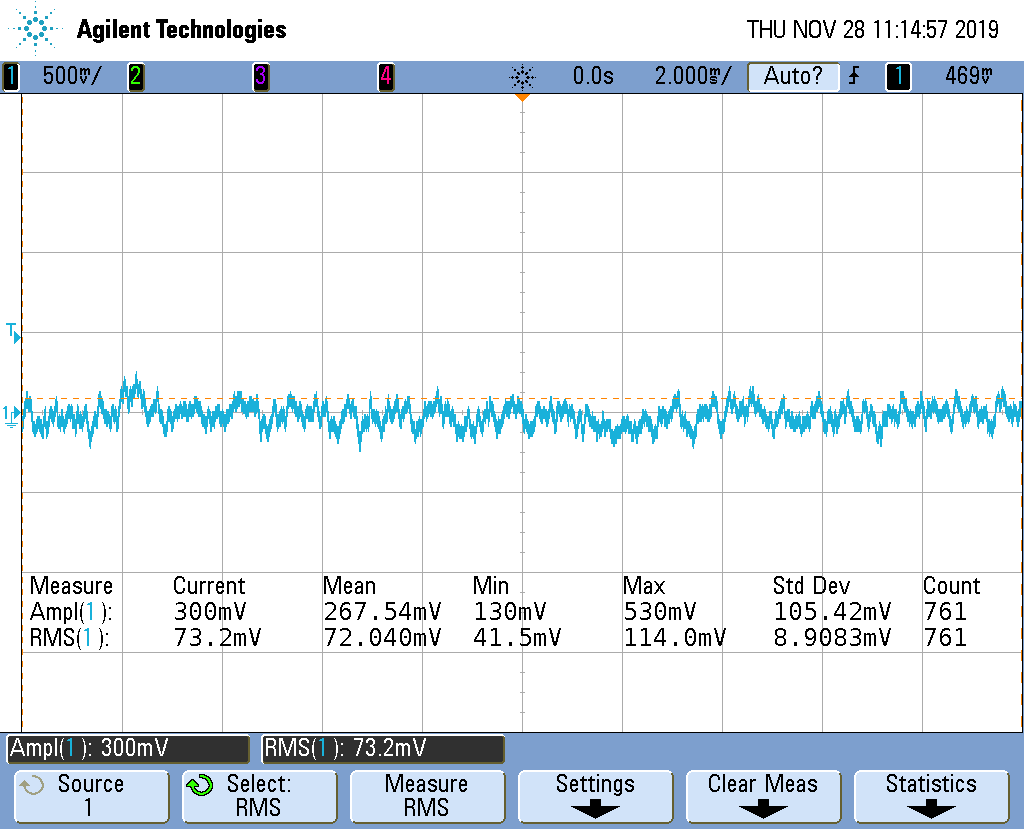
\includegraphics[width=\textwidth]{Messwerte/Rauschen/Box2_blue}
  \caption{Screenshot des Ausgangssignals von Box3.4}
\end{figure}

Aus Abbildung 9 kann mithilfe einer Regressionsgeraden ein linearer Zusammenhang zwischen Rauschleistung und
Grenzfrequenz festgestellt werden. Die Rauschleistung wurde jeweils auf die
Leistung des Eingangssignals (siehe Abbildung 5) normiert.

\begin{figure}[H]
	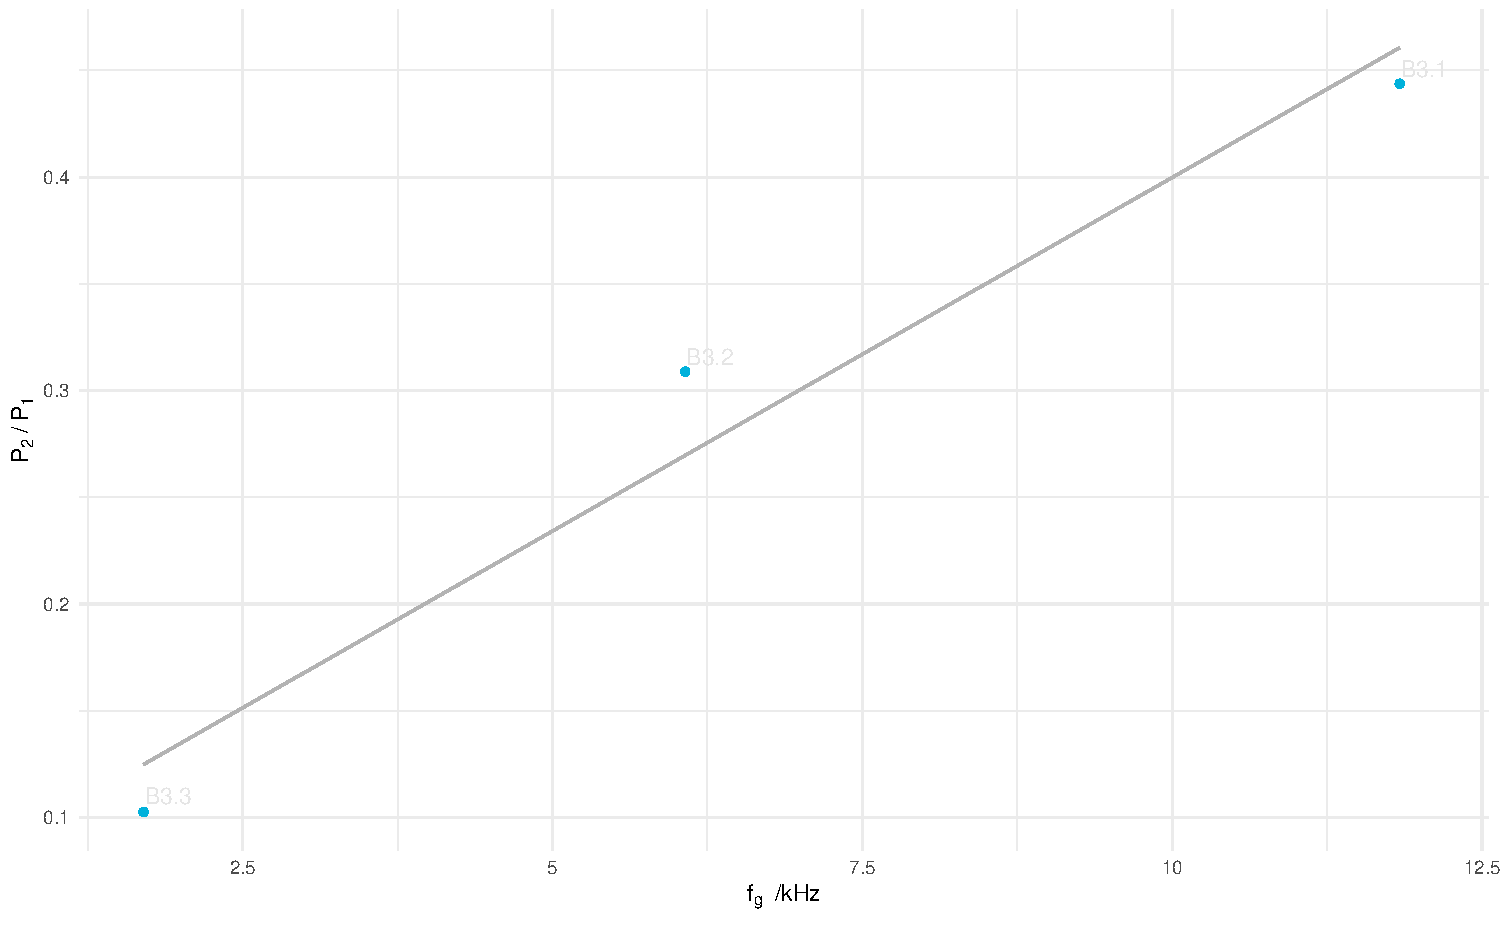
\includegraphics[width=\textwidth]{Messwerte/Rauschen/rauschleistung}
  \caption{Zusammenhang von Rauschleistung und Grenzfrequenz des Tiefpassfilters}
\end{figure}

Das Ergebnis ist sinnvoll, denn wenn man davon ausgeht, dass weißes Rauschen
ein konstantes Leistungsdichtespektrum, also gleiche Energie bei jeder Frequenz,
aufweist, und man mit Erhöhung der Grenzfrequenz mehr Frequenzanteile im Signal
zulässt, dann wird auch die Energie des Rauschens pro Zeiteinheit, also dessen
Leistung, mit der Grenzfrequenz steigen. 

\end{document}
